% Options for packages loaded elsewhere
\PassOptionsToPackage{unicode}{hyperref}
\PassOptionsToPackage{hyphens}{url}
%
\documentclass[
]{book}
\usepackage{amsmath,amssymb}
\usepackage{iftex}
\ifPDFTeX
  \usepackage[T1]{fontenc}
  \usepackage[utf8]{inputenc}
  \usepackage{textcomp} % provide euro and other symbols
\else % if luatex or xetex
  \usepackage{unicode-math} % this also loads fontspec
  \defaultfontfeatures{Scale=MatchLowercase}
  \defaultfontfeatures[\rmfamily]{Ligatures=TeX,Scale=1}
\fi
\usepackage{lmodern}
\ifPDFTeX\else
  % xetex/luatex font selection
\fi
% Use upquote if available, for straight quotes in verbatim environments
\IfFileExists{upquote.sty}{\usepackage{upquote}}{}
\IfFileExists{microtype.sty}{% use microtype if available
  \usepackage[]{microtype}
  \UseMicrotypeSet[protrusion]{basicmath} % disable protrusion for tt fonts
}{}
\makeatletter
\@ifundefined{KOMAClassName}{% if non-KOMA class
  \IfFileExists{parskip.sty}{%
    \usepackage{parskip}
  }{% else
    \setlength{\parindent}{0pt}
    \setlength{\parskip}{6pt plus 2pt minus 1pt}}
}{% if KOMA class
  \KOMAoptions{parskip=half}}
\makeatother
\usepackage{xcolor}
\usepackage{color}
\usepackage{fancyvrb}
\newcommand{\VerbBar}{|}
\newcommand{\VERB}{\Verb[commandchars=\\\{\}]}
\DefineVerbatimEnvironment{Highlighting}{Verbatim}{commandchars=\\\{\}}
% Add ',fontsize=\small' for more characters per line
\usepackage{framed}
\definecolor{shadecolor}{RGB}{248,248,248}
\newenvironment{Shaded}{\begin{snugshade}}{\end{snugshade}}
\newcommand{\AlertTok}[1]{\textcolor[rgb]{0.94,0.16,0.16}{#1}}
\newcommand{\AnnotationTok}[1]{\textcolor[rgb]{0.56,0.35,0.01}{\textbf{\textit{#1}}}}
\newcommand{\AttributeTok}[1]{\textcolor[rgb]{0.13,0.29,0.53}{#1}}
\newcommand{\BaseNTok}[1]{\textcolor[rgb]{0.00,0.00,0.81}{#1}}
\newcommand{\BuiltInTok}[1]{#1}
\newcommand{\CharTok}[1]{\textcolor[rgb]{0.31,0.60,0.02}{#1}}
\newcommand{\CommentTok}[1]{\textcolor[rgb]{0.56,0.35,0.01}{\textit{#1}}}
\newcommand{\CommentVarTok}[1]{\textcolor[rgb]{0.56,0.35,0.01}{\textbf{\textit{#1}}}}
\newcommand{\ConstantTok}[1]{\textcolor[rgb]{0.56,0.35,0.01}{#1}}
\newcommand{\ControlFlowTok}[1]{\textcolor[rgb]{0.13,0.29,0.53}{\textbf{#1}}}
\newcommand{\DataTypeTok}[1]{\textcolor[rgb]{0.13,0.29,0.53}{#1}}
\newcommand{\DecValTok}[1]{\textcolor[rgb]{0.00,0.00,0.81}{#1}}
\newcommand{\DocumentationTok}[1]{\textcolor[rgb]{0.56,0.35,0.01}{\textbf{\textit{#1}}}}
\newcommand{\ErrorTok}[1]{\textcolor[rgb]{0.64,0.00,0.00}{\textbf{#1}}}
\newcommand{\ExtensionTok}[1]{#1}
\newcommand{\FloatTok}[1]{\textcolor[rgb]{0.00,0.00,0.81}{#1}}
\newcommand{\FunctionTok}[1]{\textcolor[rgb]{0.13,0.29,0.53}{\textbf{#1}}}
\newcommand{\ImportTok}[1]{#1}
\newcommand{\InformationTok}[1]{\textcolor[rgb]{0.56,0.35,0.01}{\textbf{\textit{#1}}}}
\newcommand{\KeywordTok}[1]{\textcolor[rgb]{0.13,0.29,0.53}{\textbf{#1}}}
\newcommand{\NormalTok}[1]{#1}
\newcommand{\OperatorTok}[1]{\textcolor[rgb]{0.81,0.36,0.00}{\textbf{#1}}}
\newcommand{\OtherTok}[1]{\textcolor[rgb]{0.56,0.35,0.01}{#1}}
\newcommand{\PreprocessorTok}[1]{\textcolor[rgb]{0.56,0.35,0.01}{\textit{#1}}}
\newcommand{\RegionMarkerTok}[1]{#1}
\newcommand{\SpecialCharTok}[1]{\textcolor[rgb]{0.81,0.36,0.00}{\textbf{#1}}}
\newcommand{\SpecialStringTok}[1]{\textcolor[rgb]{0.31,0.60,0.02}{#1}}
\newcommand{\StringTok}[1]{\textcolor[rgb]{0.31,0.60,0.02}{#1}}
\newcommand{\VariableTok}[1]{\textcolor[rgb]{0.00,0.00,0.00}{#1}}
\newcommand{\VerbatimStringTok}[1]{\textcolor[rgb]{0.31,0.60,0.02}{#1}}
\newcommand{\WarningTok}[1]{\textcolor[rgb]{0.56,0.35,0.01}{\textbf{\textit{#1}}}}
\usepackage{longtable,booktabs,array}
\usepackage{calc} % for calculating minipage widths
% Correct order of tables after \paragraph or \subparagraph
\usepackage{etoolbox}
\makeatletter
\patchcmd\longtable{\par}{\if@noskipsec\mbox{}\fi\par}{}{}
\makeatother
% Allow footnotes in longtable head/foot
\IfFileExists{footnotehyper.sty}{\usepackage{footnotehyper}}{\usepackage{footnote}}
\makesavenoteenv{longtable}
\usepackage{graphicx}
\makeatletter
\def\maxwidth{\ifdim\Gin@nat@width>\linewidth\linewidth\else\Gin@nat@width\fi}
\def\maxheight{\ifdim\Gin@nat@height>\textheight\textheight\else\Gin@nat@height\fi}
\makeatother
% Scale images if necessary, so that they will not overflow the page
% margins by default, and it is still possible to overwrite the defaults
% using explicit options in \includegraphics[width, height, ...]{}
\setkeys{Gin}{width=\maxwidth,height=\maxheight,keepaspectratio}
% Set default figure placement to htbp
\makeatletter
\def\fps@figure{htbp}
\makeatother
\setlength{\emergencystretch}{3em} % prevent overfull lines
\providecommand{\tightlist}{%
  \setlength{\itemsep}{0pt}\setlength{\parskip}{0pt}}
\setcounter{secnumdepth}{5}
\usepackage{booktabs}
\ifLuaTeX
  \usepackage{selnolig}  % disable illegal ligatures
\fi
\usepackage[]{natbib}
\bibliographystyle{plainnat}
\IfFileExists{bookmark.sty}{\usepackage{bookmark}}{\usepackage{hyperref}}
\IfFileExists{xurl.sty}{\usepackage{xurl}}{} % add URL line breaks if available
\urlstyle{same}
\hypersetup{
  pdftitle={Tutorial 1: Intro to R},
  pdfauthor={Heather Kropp},
  hidelinks,
  pdfcreator={LaTeX via pandoc}}

\title{Tutorial 1: Intro to R}
\author{Heather Kropp}
\date{2023-08-07}

\usepackage{amsthm}
\newtheorem{theorem}{Theorem}[chapter]
\newtheorem{lemma}{Lemma}[chapter]
\newtheorem{corollary}{Corollary}[chapter]
\newtheorem{proposition}{Proposition}[chapter]
\newtheorem{conjecture}{Conjecture}[chapter]
\theoremstyle{definition}
\newtheorem{definition}{Definition}[chapter]
\theoremstyle{definition}
\newtheorem{example}{Example}[chapter]
\theoremstyle{definition}
\newtheorem{exercise}{Exercise}[chapter]
\theoremstyle{definition}
\newtheorem{hypothesis}{Hypothesis}[chapter]
\theoremstyle{remark}
\newtheorem*{remark}{Remark}
\newtheorem*{solution}{Solution}
\begin{document}
\maketitle

{
\setcounter{tocdepth}{1}
\tableofcontents
}
\hypertarget{about}{%
\chapter{About}\label{about}}

This is a \emph{sample} book written in \textbf{Markdown}. You can use anything that Pandoc's Markdown supports; for example, a math equation \(a^2 + b^2 = c^2\).

\hypertarget{usage}{%
\section{Usage}\label{usage}}

Each \textbf{bookdown} chapter is an .Rmd file, and each .Rmd file can contain one (and only one) chapter. A chapter \emph{must} start with a first-level heading: \texttt{\#\ A\ good\ chapter}, and can contain one (and only one) first-level heading.

Use second-level and higher headings within chapters like: \texttt{\#\#\ A\ short\ section} or \texttt{\#\#\#\ An\ even\ shorter\ section}.

The \texttt{index.Rmd} file is required, and is also your first book chapter. It will be the homepage when you render the book.

\hypertarget{render-book}{%
\section{Render book}\label{render-book}}

You can render the HTML version of this example book without changing anything:

\begin{enumerate}
\def\labelenumi{\arabic{enumi}.}
\item
  Find the \textbf{Build} pane in the RStudio IDE, and
\item
  Click on \textbf{Build Book}, then select your output format, or select ``All formats'' if you'd like to use multiple formats from the same book source files.
\end{enumerate}

Or build the book from the R console:

\begin{Shaded}
\begin{Highlighting}[]
\NormalTok{bookdown}\SpecialCharTok{::}\FunctionTok{render\_book}\NormalTok{()}
\end{Highlighting}
\end{Shaded}

To render this example to PDF as a \texttt{bookdown::pdf\_book}, you'll need to install XeLaTeX. You are recommended to install TinyTeX (which includes XeLaTeX): \url{https://yihui.org/tinytex/}.

\hypertarget{preview-book}{%
\section{Preview book}\label{preview-book}}

As you work, you may start a local server to live preview this HTML book. This preview will update as you edit the book when you save individual .Rmd files. You can start the server in a work session by using the RStudio add-in ``Preview book'', or from the R console:

\begin{Shaded}
\begin{Highlighting}[]
\NormalTok{bookdown}\SpecialCharTok{::}\FunctionTok{serve\_book}\NormalTok{()}
\end{Highlighting}
\end{Shaded}

\hypertarget{envst-206-intro-to-environmental-data-hamilton-college}{%
\subsubsection{\texorpdfstring{\emph{ENVST 206: Intro to Environmental Data, Hamilton College}}{ENVST 206: Intro to Environmental Data, Hamilton College}}\label{envst-206-intro-to-environmental-data-hamilton-college}}

\hypertarget{learning-objectives}{%
\section{Learning objectives}\label{learning-objectives}}

\hypertarget{learn-about-rstudio-cloud}{%
\subsubsection{1. Learn about RStudio Cloud}\label{learn-about-rstudio-cloud}}

\hypertarget{introduction-to-r-rstudio}{%
\subsubsection{2. Introduction to R \& Rstudio}\label{introduction-to-r-rstudio}}

\hypertarget{learn-the-basics}{%
\subsubsection{3. Learn the basics}\label{learn-the-basics}}

\hypertarget{first-some-terms}{%
\section{First some terms:}\label{first-some-terms}}

\textbf{R}: a statistical programming software that can be used to analyze data

\textbf{RStudio}: a user friendly interface for running R

\textbf{Cloud computing} a remote computer that you access using your browser.

\textbf{RStudio Cloud} runs RStudio in a cloud computing environment. Each assignment or activity you do will open up in this virtual computer.

\hypertarget{getting-to-know-rstudio-cloud}{%
\section{Getting to know Rstudio Cloud}\label{getting-to-know-rstudio-cloud}}

RStudio Cloud helps create a standardized computing environment for us as a class that is specifically meant to support working in R. This means that you can access the same computing environment and you only need to run a web browser on a personal or Hamilton computer. This will allow coursework to be readily completed from any computer whether you are on or off campus. It also means that you don't have to worry about installing R or storing data on your own personal computer.

You will have received an invitation to join the ENVST206-F21 \textbf{workspace} on RStudio Cloud through your Hamilton email. Once you have joined the workspace, you can access the projects section. A \textbf{project} is a collection of related R files and data. \textbf{Assignments} are projects that are set up to be read only and you will make your own copy when you open it. Your copy will automatically be set up with your user profile once you save it. You will see a blue box next to the project name indicating that it is an assignment. You will have the option to start the assignment for the first time or continue if you already started it.


\includegraphics[width=0.5\textwidth,height=\textheight]{/Users/hkropp/Documents/GitHub/Intro_EnvData/bookdown/IntroEnvData/photos/tutorial_1/Assignment.png}

Once you open the assignment, you will see an interface that looks something like this:

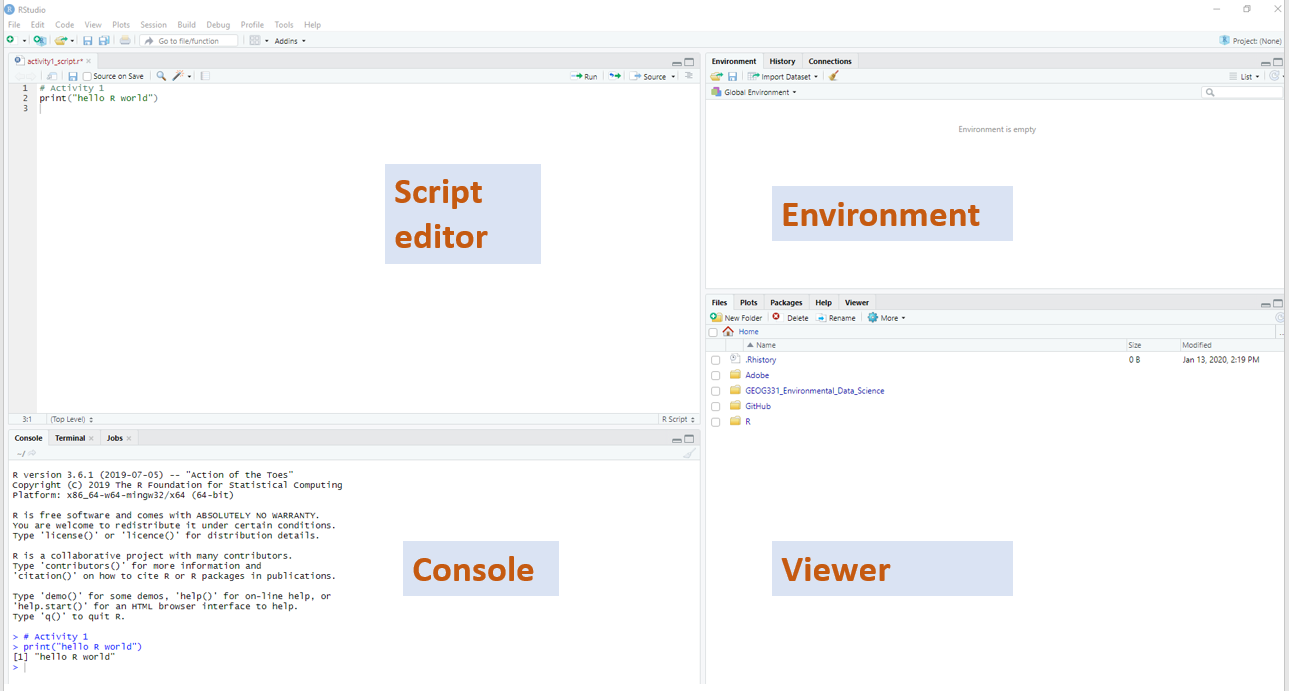
\includegraphics{/Users/hkropp/Documents/GitHub/Intro_EnvData/bookdown/IntroEnvData/photos/tutorial_1/Rstudio.png}

The Rstudio interface has 4 main components: \textbf{1. script window, 2. console, 3. environment, 4. viewer \& information tabs}. In the next section, you will learn more about each of these parts of the interface.

\hypertarget{introduction-to-r-rstudio-1}{%
\section{Introduction to R \& RStudio}\label{introduction-to-r-rstudio-1}}

R is essentially a giant calculator with many options for plotting and built in functions for data analysis. The \textbf{console} runs your R code. It's the calculator! You can type code into the console and it will run. However, you won't be able to access that code later, just like many calculators. That's why we use \textbf{scripts}.

R scripts allow you to save code in a text file to run in R. R scripts all have a .r extension. By itself, the script will do nothing. You need to actually tell R to run your code in the console. When you first open a Rstudio, there is often a blank work space with just the console unless I have set up some existing files to open for you. You can tell you are looking at the console by checking the tabs, and you will see information about your R version at the start.

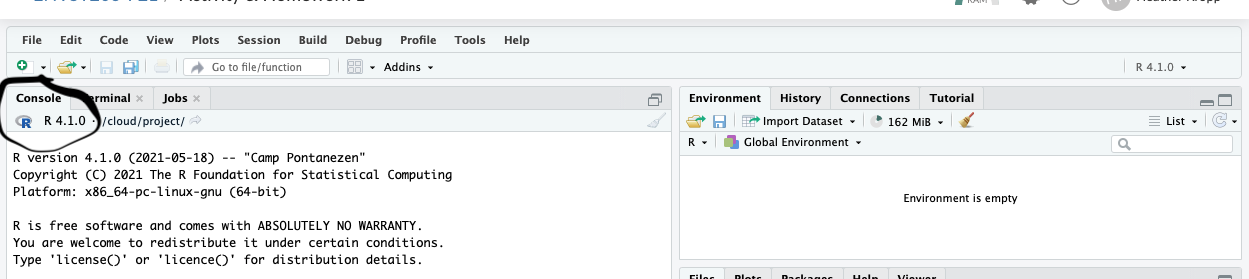
\includegraphics[width=1\textwidth,height=\textheight]{/Users/hkropp/Documents/GitHub/Intro_EnvData/bookdown/IntroEnvData/photos/tutorial_1/console open.png}

New scripts can be created by going to \emph{New File} and clicking on Rscript. If you wanted to open an existing Rscript, you can go to \emph{Open File}.

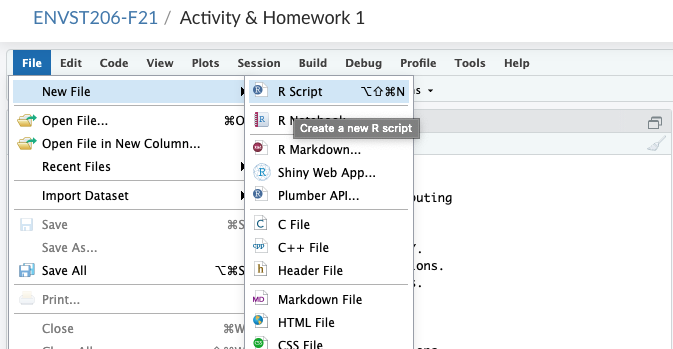
\includegraphics[width=0.5\textwidth,height=\textheight]{/Users/hkropp/Documents/GitHub/Intro_EnvData/bookdown/IntroEnvData/photos/tutorial_1/new script.png}

Clicking a new script will prompt you to save into the file system created in our project computer:

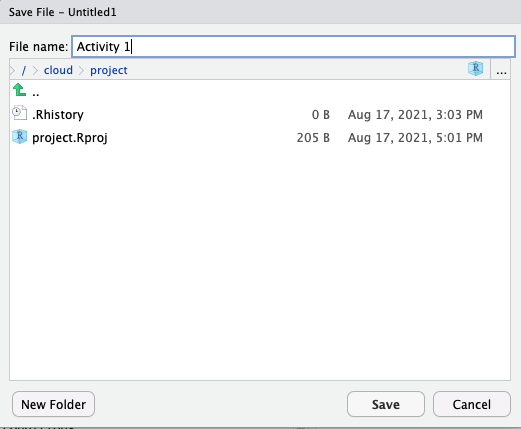
\includegraphics[width=0.5\textwidth,height=\textheight]{/Users/hkropp/Documents/GitHub/Intro_EnvData/bookdown/IntroEnvData/photos/tutorial_1/save prompt.png}

You will see that saving your script will create a new file in the Files tab in the bottom right corner. This tab will be important when we start working with more data files.

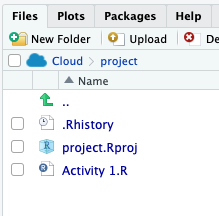
\includegraphics[width=0.25\textwidth,height=\textheight]{/Users/hkropp/Documents/GitHub/Intro_EnvData/bookdown/IntroEnvData/photos/tutorial_1/file system.png}

The script opens up above the console and is ready for you to code!

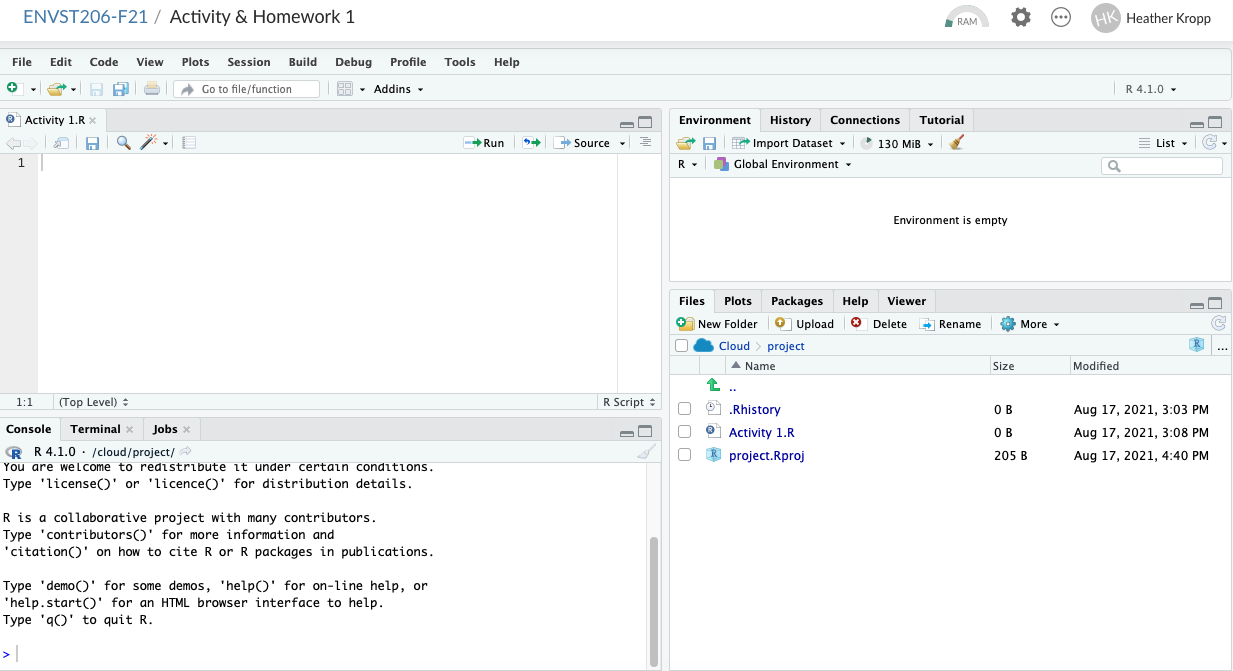
\includegraphics[width=0.75\textwidth,height=\textheight]{/Users/hkropp/Documents/GitHub/Intro_EnvData/bookdown/IntroEnvData/photos/tutorial_1/Rstudio open.png}

You can get a better idea for the script/console set up by writing a simple line of code in the script and running it. Using the function \texttt{print}, any text within the function will be returned in the console. You can also use hashes \texttt{\#} to make a \textbf{comment} so that you can document code. Let's take a look at how this works before getting into the details. Here is the code in my script:

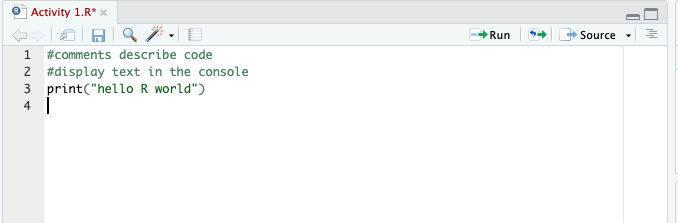
\includegraphics[width=0.5\textwidth,height=\textheight]{/Users/hkropp/Documents/GitHub/Intro_EnvData/bookdown/IntroEnvData/photos/tutorial_1/first code.png}

Nothing happens with this code until I run it in the console.You can run a line of code clicking in the line or a selection of code by highlighting it and pressing the run button (shown in the black circle).

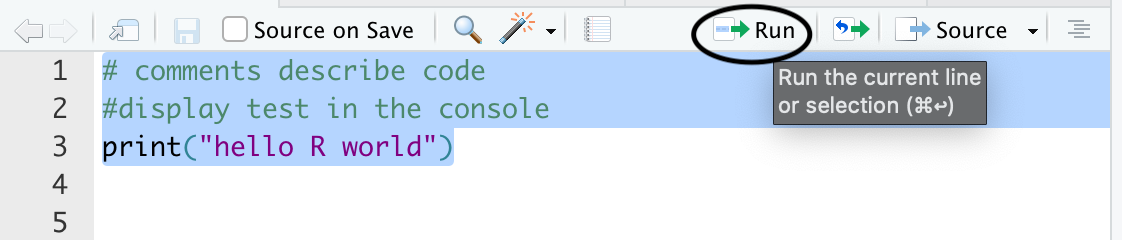
\includegraphics[width=0.5\textwidth,height=\textheight]{/Users/hkropp/Documents/GitHub/Intro_EnvData/bookdown/IntroEnvData/photos/tutorial_1/running.png}

There's a few things to pay attention to in the console when you run code. The \texttt{\textgreater{}} symbol always indicates a new line of code. The \texttt{+} symbol means your line of code has not ended and will continue on to the next line. Your results will have numbers in brackets to describe the output. \texttt{{[}1{]}} indicates the start of the output.

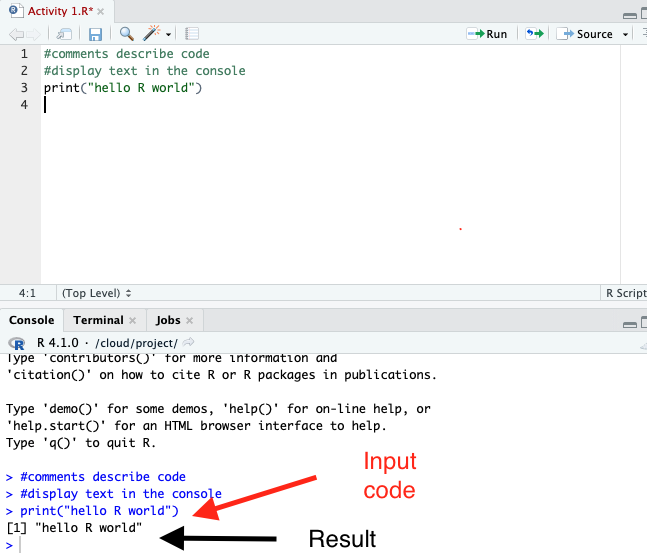
\includegraphics[width=0.5\textwidth,height=\textheight]{/Users/hkropp/Documents/GitHub/Intro_EnvData/bookdown/IntroEnvData/photos/tutorial_1/Running explain.png}

Any variables run in the console are part of your \textbf{working environment}. Variables allow you to refer to the same data or calculations throughout your current R session the computer's temporary memory. You'll learn more about R code in the next section to fully understand the utility of the working environment.


\includegraphics{_main_files/figure-latex/unnamed-chunk-6-1.pdf}

\hypertarget{r-basics}{%
\section{R basics}\label{r-basics}}

\hypertarget{a-fancy-calculator}{%
\subsection{\texorpdfstring{\emph{A fancy calculator}}{A fancy calculator}}\label{a-fancy-calculator}}

Since R is just like a sophisticated calculator, you can read in numerical operations and will get the calculations as output. Type a few different operations like the one below that follow typical mathematical notation on a keyboard. Note I've included both the code (grey boxes) and outputs (blue boxes) here for an example.

\begin{Shaded}
\begin{Highlighting}[]
\CommentTok{\# remember this is a comment so it won\textquotesingle{}t do anything. R just ignores it.}
\CommentTok{\# you need to use these to document code and write notes}
\CommentTok{\# 6 raised to the 6 power}
\DecValTok{6}\SpecialCharTok{\^{}}\DecValTok{6}
\end{Highlighting}
\end{Shaded}

\begin{Shaded}
\begin{Highlighting}[]
\NormalTok{[1] 46656}
\end{Highlighting}
\end{Shaded}

\begin{Shaded}
\begin{Highlighting}[]
\CommentTok{\# 5 plus 210}
\DecValTok{5}\SpecialCharTok{+}\DecValTok{210}
\end{Highlighting}
\end{Shaded}

\begin{Shaded}
\begin{Highlighting}[]
\NormalTok{[1] 215}
\end{Highlighting}
\end{Shaded}

\begin{Shaded}
\begin{Highlighting}[]
\CommentTok{\# 3 minus 10}
\DecValTok{3{-}10}
\end{Highlighting}
\end{Shaded}

\begin{Shaded}
\begin{Highlighting}[]
\NormalTok{[1] {-}7}
\end{Highlighting}
\end{Shaded}

\hypertarget{variables}{%
\subsection{\texorpdfstring{\emph{Variables}}{Variables}}\label{variables}}

Typing in calculations can quickly become redundant and difficult when you have many observations. Creating a \textbf{variable} allows you to refer to the same object by typing its name. You can create a variable by first typing a name, then typing the assigner \texttt{\textless{}-} (\texttt{=} also works, but is not R convention). Anything to the right of the assigner will be refered to with the name you give. Below is an example where I know I will want to use the number 244435600 many times so I will give it a shorter, easier to remember name.

\begin{Shaded}
\begin{Highlighting}[]
\CommentTok{\# name my number}
\NormalTok{aNumber }\OtherTok{\textless{}{-}} \DecValTok{244435600}
\CommentTok{\# multiply my number by 5}
\DecValTok{5}\SpecialCharTok{*}\NormalTok{aNumber}
\end{Highlighting}
\end{Shaded}

\begin{Shaded}
\begin{Highlighting}[]
\NormalTok{[1] 1222178000}
\end{Highlighting}
\end{Shaded}

\begin{Shaded}
\begin{Highlighting}[]
\CommentTok{\# divide my number by 2}
\NormalTok{aNumber}\SpecialCharTok{/}\DecValTok{2}
\end{Highlighting}
\end{Shaded}

\begin{Shaded}
\begin{Highlighting}[]
\NormalTok{[1] 122217800}
\end{Highlighting}
\end{Shaded}

\hypertarget{vectors}{%
\subsection{\texorpdfstring{\emph{Vectors}}{Vectors}}\label{vectors}}

A vector is a one dimensional array of data. You can make a vector in R using the function \texttt{c()}. \texttt{c} stands for combine values into a vector where each value is separated by a comma. For example, here's a vector with the elevation of the three highest peaks in the Adirondacks.

\begin{Shaded}
\begin{Highlighting}[]
\CommentTok{\# make a vector of numbers}
\CommentTok{\# elevation in ft}
\NormalTok{peaks }\OtherTok{\textless{}{-}} \FunctionTok{c}\NormalTok{(}\DecValTok{5344}\NormalTok{,}\DecValTok{5114}\NormalTok{,}\DecValTok{4960}\NormalTok{)}
\end{Highlighting}
\end{Shaded}

You will notice that both functions \texttt{print} and \texttt{c} are text followed by parentheses. This is a detail to pay attention to for the R \textbf{syntax}. Syntax refers to the rulues and structure of a coding language. What you learned about \texttt{\#} and \texttt{\textless{}-} are examples of R syntax since these symbols have a specific meaning. Any time you see the format \texttt{anyName()} you can know this is a \textbf{function}. Functions are a key part of R. You already used functions by runnidn \texttt{c} and \texttt{print}. They expect certain inputs called \textbf{arguments} (like our numbers in the \emph{c} function used to create peaks vector). Functions will also perform a task that saves you a lot of extra coding. You can immediately see the utility of functions by running summary statistics functions like: \texttt{mean} (average value of a vector), \texttt{min} (minimum value in a vector), \texttt{max} (maximum value in a vector).

\begin{Shaded}
\begin{Highlighting}[]
\CommentTok{\# calculate the mean of peaks}
\FunctionTok{mean}\NormalTok{(peaks)}
\end{Highlighting}
\end{Shaded}

\begin{Shaded}
\begin{Highlighting}[]
\NormalTok{[1] 5139.333}
\end{Highlighting}
\end{Shaded}

\begin{Shaded}
\begin{Highlighting}[]
\CommentTok{\# calculate the minimum peak}
\FunctionTok{min}\NormalTok{(peaks)}
\end{Highlighting}
\end{Shaded}

\begin{Shaded}
\begin{Highlighting}[]
\NormalTok{[1] 4960}
\end{Highlighting}
\end{Shaded}

\begin{Shaded}
\begin{Highlighting}[]
\CommentTok{\# save the maximum as a variable}
\NormalTok{maxPeak }\OtherTok{\textless{}{-}} \FunctionTok{max}\NormalTok{(peaks)}
\end{Highlighting}
\end{Shaded}

When you create a variable like \texttt{maxPeak} there is no output shown in the console. It can look alarming, but it is actually a good sign! It means your code worked! The variable \texttt{maxPeak} was simply created. You can always run the name of variable with nothing else to get a print out:

\begin{Shaded}
\begin{Highlighting}[]
\NormalTok{maxPeak}
\end{Highlighting}
\end{Shaded}

\begin{Shaded}
\begin{Highlighting}[]
\NormalTok{[1] 5344}
\end{Highlighting}
\end{Shaded}

If you look to your environment section of RStudio, you will see \texttt{peaks} and \texttt{maxPeak} are shown in the global environment. \texttt{peaks} is a data type \textbf{numeric} and it has 3 total objects. Numeric data are all numbers and can include numbers on both sides of the decimal. This is where watching your environment section is useful to check that your code is working as you expect.

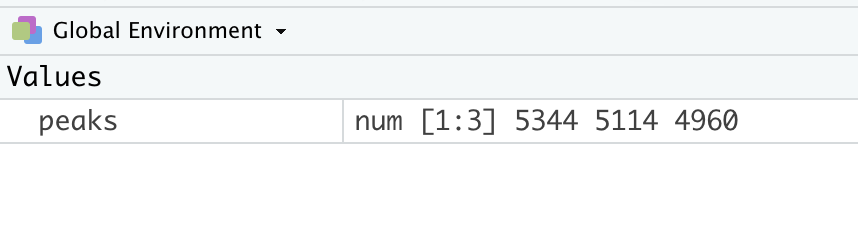
\includegraphics[width=0.5\textwidth,height=\textheight]{/Users/hkropp/Documents/GitHub/Intro_EnvData/Week01/photos/environment.png}

You can now do calculations on each object in your vector. For example, if you want to convert the peak elevation to meters, you simply need to type in one calculation. You'll notice, this calculation was not assigned as a named variable, and a vector of output is returned but not stored in the environment.

\begin{Shaded}
\begin{Highlighting}[]
\CommentTok{\# convert to meters}
\NormalTok{peaks}\SpecialCharTok{/}\FloatTok{3.281}
\end{Highlighting}
\end{Shaded}

\begin{Shaded}
\begin{Highlighting}[]
\NormalTok{[1] 1628.772 1558.671 1511.734}
\end{Highlighting}
\end{Shaded}

You can also apply vector operations on vectors that are the same length and a calculation for the element in each vector makes sense. For example, I can make a vector of the prominence (height from the base) and calculate the difference to find the difference between the elevation of the mountain and the prominence.

\begin{Shaded}
\begin{Highlighting}[]
\CommentTok{\# prominence in ft}
\NormalTok{prom }\OtherTok{\textless{}{-}} \FunctionTok{c}\NormalTok{(}\DecValTok{4914}\NormalTok{,}\DecValTok{2100}\NormalTok{,}\DecValTok{840}\NormalTok{)}
\CommentTok{\# difference between height and prominence}
\NormalTok{peaks }\SpecialCharTok{{-}}\NormalTok{ prom}
\end{Highlighting}
\end{Shaded}

\begin{Shaded}
\begin{Highlighting}[]
\NormalTok{[1]  430 3014 4120}
\end{Highlighting}
\end{Shaded}

You can also make vectors with other types of data beyond numeric. R supports data types such as dates, character strings, and integers. A \textbf{character} is any mixture of letters, numbers, and symbols. You can't apply mathematical calculations to character. You can set up a vector of the mountain names by using quotes around each character element in the vector:

\begin{Shaded}
\begin{Highlighting}[]
\CommentTok{\# quotes denote a character data type}
\NormalTok{peakNames }\OtherTok{\textless{}{-}} \FunctionTok{c}\NormalTok{(}\StringTok{"Mount Marcy"}\NormalTok{, }\StringTok{"Algonquin Peak"}\NormalTok{, }\StringTok{"Mount Haystack"}\NormalTok{)}
\end{Highlighting}
\end{Shaded}

You can \textbf{subset} a vector using \texttt{{[}{]}} syntax. If you want to refer to just the first item in a vector, you can subset as follows:

\begin{Shaded}
\begin{Highlighting}[]
\CommentTok{\# elevation of first peak}
\NormalTok{peaks[}\DecValTok{1}\NormalTok{]}
\end{Highlighting}
\end{Shaded}

\begin{Shaded}
\begin{Highlighting}[]
\NormalTok{[1] 5344}
\end{Highlighting}
\end{Shaded}

\hypertarget{data-frames}{%
\subsection{\texorpdfstring{\emph{Data frames}}{Data frames}}\label{data-frames}}

The final basic type of data that will be useful to keep in mind is a data frame. \textbf{Data frames} are a matrix with column names and sometimes row names. All observations in a row are associated. Each column will have the same type of data. For example, you can make a dataframe with all of the high peaks information using the `data.frame' function. For the \texttt{data.frame} arguments, you specify each vector to include as a column and the name of the column (left side of each equal sign).

\begin{Shaded}
\begin{Highlighting}[]
\CommentTok{\# make a datframee}
\CommentTok{\# you must include the column name = data vector}
\CommentTok{\# seperating multiple columns with commas}
\NormalTok{highPeaks }\OtherTok{\textless{}{-}} \FunctionTok{data.frame}\NormalTok{(}\AttributeTok{elev =}\NormalTok{ peaks,}
                        \AttributeTok{prom =}\NormalTok{ prom,}
                        \AttributeTok{name =}\NormalTok{ peakNames)}
\end{Highlighting}
\end{Shaded}

A helpful way to check that your code ran as expected is to track the objects in your global environment. Vectors show up under \emph{values} and data frames are shown under \emph{data}. If you click the blue arrow button you will get a preview of the data frame.

You can subset a data frame using the \texttt{{[}{]}} syntax, but you need to account for the two dimensional nature of data frames. If you are taking all observations for a row or column, it can simply be left empty.

\begin{Shaded}
\begin{Highlighting}[]
\CommentTok{\# subset 2 row in highPeaks}
\NormalTok{highPeaks[}\DecValTok{2}\NormalTok{,]}
\end{Highlighting}
\end{Shaded}

\begin{Shaded}
\begin{Highlighting}[]
\NormalTok{  elev prom           name}
\NormalTok{2 5114 2100 Algonquin Peak}
\end{Highlighting}
\end{Shaded}

\begin{Shaded}
\begin{Highlighting}[]
\CommentTok{\# view only the names column}
\NormalTok{highPeaks[,}\DecValTok{3}\NormalTok{]}
\end{Highlighting}
\end{Shaded}

\begin{Shaded}
\begin{Highlighting}[]
\NormalTok{[1] "Mount Marcy"    "Algonquin Peak" "Mount Haystack"}
\end{Highlighting}
\end{Shaded}

\begin{Shaded}
\begin{Highlighting}[]
\CommentTok{\# look at elevation for 3rd highest mountain}
\NormalTok{highPeaks[}\DecValTok{1}\NormalTok{,}\DecValTok{3}\NormalTok{]}
\end{Highlighting}
\end{Shaded}

\begin{Shaded}
\begin{Highlighting}[]
\NormalTok{[1] "Mount Marcy"}
\end{Highlighting}
\end{Shaded}


\includegraphics{_main_files/figure-latex/unnamed-chunk-18-1.pdf}

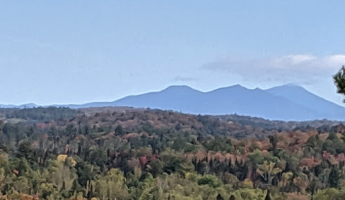
\includegraphics[width=0.4\textwidth,height=\textheight]{/Users/hkropp/Documents/GitHub/Intro_EnvData/bookdown/IntroEnvData/photos/tutorial_1/peaks2.png}

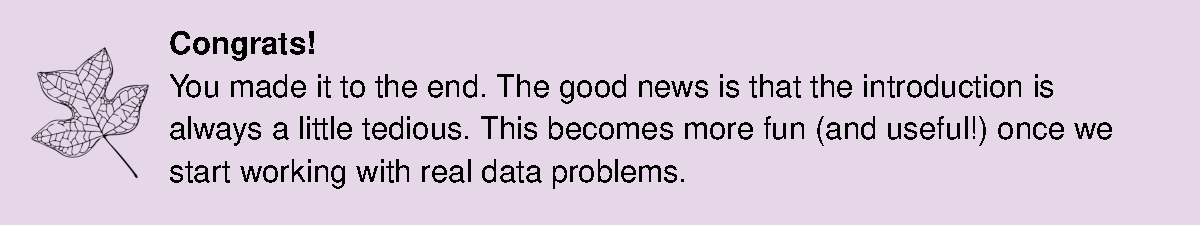
\includegraphics{_main_files/figure-latex/unnamed-chunk-19-1.pdf}

\hypertarget{cross}{%
\chapter{Cross-references}\label{cross}}

Cross-references make it easier for your readers to find and link to elements in your book.

\hypertarget{chapters-and-sub-chapters}{%
\section{Chapters and sub-chapters}\label{chapters-and-sub-chapters}}

There are two steps to cross-reference any heading:

\begin{enumerate}
\def\labelenumi{\arabic{enumi}.}
\tightlist
\item
  Label the heading: \texttt{\#\ Hello\ world\ \{\#nice-label\}}.

  \begin{itemize}
  \tightlist
  \item
    Leave the label off if you like the automated heading generated based on your heading title: for example, \texttt{\#\ Hello\ world} = \texttt{\#\ Hello\ world\ \{\#hello-world\}}.
  \item
    To label an un-numbered heading, use: \texttt{\#\ Hello\ world\ \{-\#nice-label\}} or \texttt{\{\#\ Hello\ world\ .unnumbered\}}.
  \end{itemize}
\item
  Next, reference the labeled heading anywhere in the text using \texttt{\textbackslash{}@ref(nice-label)}; for example, please see Chapter \ref{cross}.

  \begin{itemize}
  \tightlist
  \item
    If you prefer text as the link instead of a numbered reference use: \protect\hyperlink{cross}{any text you want can go here}.
  \end{itemize}
\end{enumerate}

\hypertarget{captioned-figures-and-tables}{%
\section{Captioned figures and tables}\label{captioned-figures-and-tables}}

Figures and tables \emph{with captions} can also be cross-referenced from elsewhere in your book using \texttt{\textbackslash{}@ref(fig:chunk-label)} and \texttt{\textbackslash{}@ref(tab:chunk-label)}, respectively.

See Figure \ref{fig:nice-fig}.

\begin{Shaded}
\begin{Highlighting}[]
\FunctionTok{par}\NormalTok{(}\AttributeTok{mar =} \FunctionTok{c}\NormalTok{(}\DecValTok{4}\NormalTok{, }\DecValTok{4}\NormalTok{, .}\DecValTok{1}\NormalTok{, .}\DecValTok{1}\NormalTok{))}
\FunctionTok{plot}\NormalTok{(pressure, }\AttributeTok{type =} \StringTok{\textquotesingle{}b\textquotesingle{}}\NormalTok{, }\AttributeTok{pch =} \DecValTok{19}\NormalTok{)}
\end{Highlighting}
\end{Shaded}

\begin{figure}

{\centering 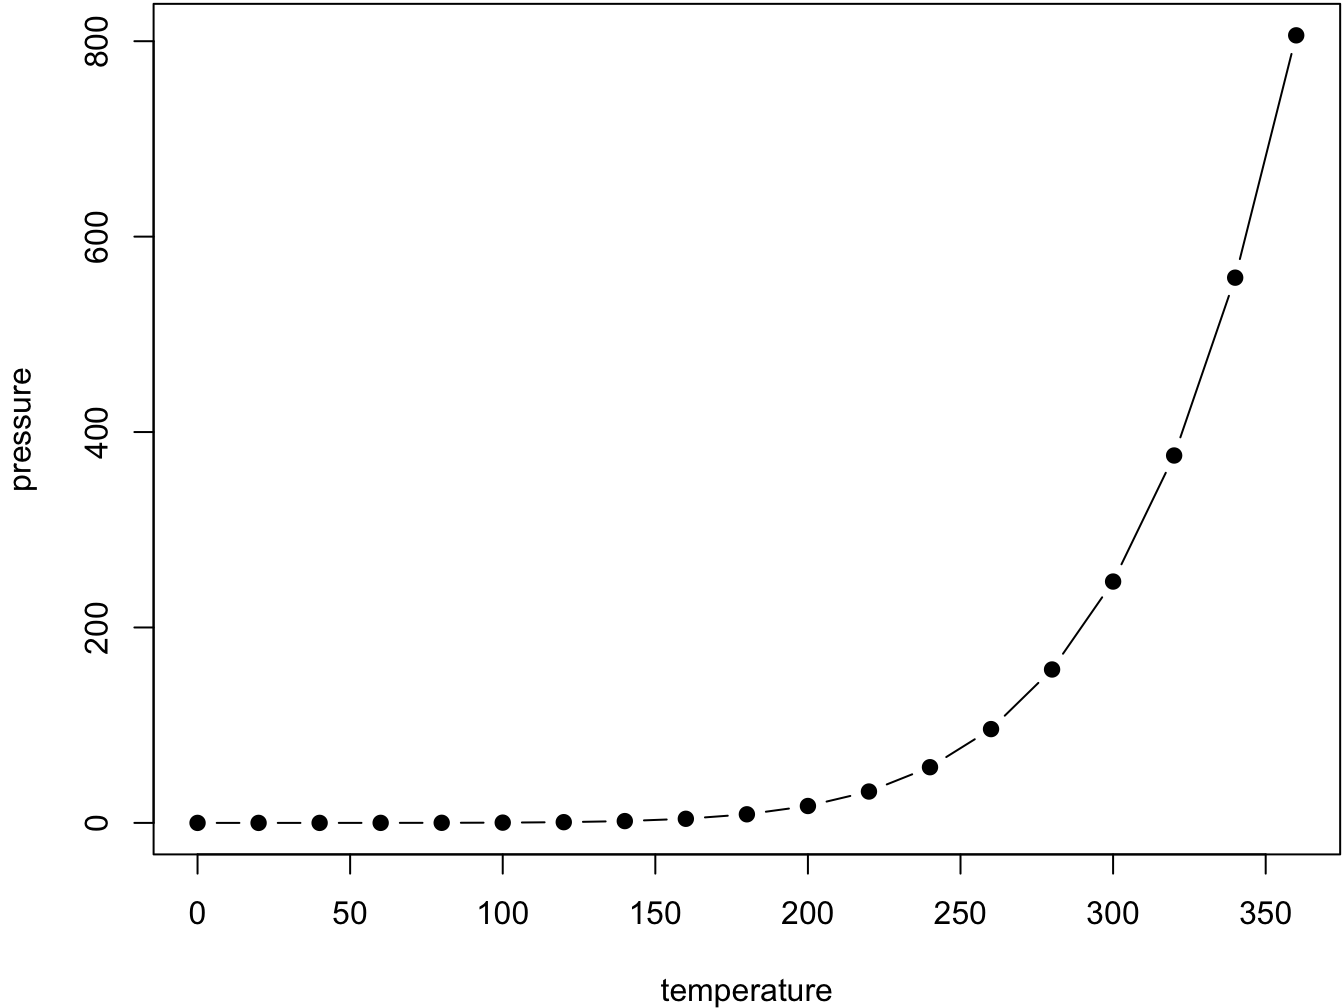
\includegraphics[width=0.8\linewidth]{_main_files/figure-latex/nice-fig-1} 

}

\caption{Here is a nice figure!}\label{fig:nice-fig}
\end{figure}

Don't miss Table \ref{tab:nice-tab}.

\begin{Shaded}
\begin{Highlighting}[]
\NormalTok{knitr}\SpecialCharTok{::}\FunctionTok{kable}\NormalTok{(}
  \FunctionTok{head}\NormalTok{(pressure, }\DecValTok{10}\NormalTok{), }\AttributeTok{caption =} \StringTok{\textquotesingle{}Here is a nice table!\textquotesingle{}}\NormalTok{,}
  \AttributeTok{booktabs =} \ConstantTok{TRUE}
\NormalTok{)}
\end{Highlighting}
\end{Shaded}

\begin{table}

\caption{\label{tab:nice-tab}Here is a nice table!}
\centering
\begin{tabular}[t]{rr}
\toprule
temperature & pressure\\
\midrule
0 & 0.0002\\
20 & 0.0012\\
40 & 0.0060\\
60 & 0.0300\\
80 & 0.0900\\
\addlinespace
100 & 0.2700\\
120 & 0.7500\\
140 & 1.8500\\
160 & 4.2000\\
180 & 8.8000\\
\bottomrule
\end{tabular}
\end{table}

\hypertarget{parts}{%
\chapter{Parts}\label{parts}}

You can add parts to organize one or more book chapters together. Parts can be inserted at the top of an .Rmd file, before the first-level chapter heading in that same file.

Add a numbered part: \texttt{\#\ (PART)\ Act\ one\ \{-\}} (followed by \texttt{\#\ A\ chapter})

Add an unnumbered part: \texttt{\#\ (PART\textbackslash{}*)\ Act\ one\ \{-\}} (followed by \texttt{\#\ A\ chapter})

Add an appendix as a special kind of un-numbered part: \texttt{\#\ (APPENDIX)\ Other\ stuff\ \{-\}} (followed by \texttt{\#\ A\ chapter}). Chapters in an appendix are prepended with letters instead of numbers.

\hypertarget{footnotes-and-citations}{%
\chapter{Footnotes and citations}\label{footnotes-and-citations}}

\hypertarget{footnotes}{%
\section{Footnotes}\label{footnotes}}

Footnotes are put inside the square brackets after a caret \texttt{\^{}{[}{]}}. Like this one \footnote{This is a footnote.}.

\hypertarget{citations}{%
\section{Citations}\label{citations}}

Reference items in your bibliography file(s) using \texttt{@key}.

For example, we are using the \textbf{bookdown} package \citep{R-bookdown} (check out the last code chunk in index.Rmd to see how this citation key was added) in this sample book, which was built on top of R Markdown and \textbf{knitr} \citep{xie2015} (this citation was added manually in an external file book.bib).
Note that the \texttt{.bib} files need to be listed in the index.Rmd with the YAML \texttt{bibliography} key.

The RStudio Visual Markdown Editor can also make it easier to insert citations: \url{https://rstudio.github.io/visual-markdown-editing/\#/citations}

\hypertarget{blocks}{%
\chapter{Blocks}\label{blocks}}

\hypertarget{equations}{%
\section{Equations}\label{equations}}

Here is an equation.

\begin{equation} 
  f\left(k\right) = \binom{n}{k} p^k\left(1-p\right)^{n-k}
  \label{eq:binom}
\end{equation}

You may refer to using \texttt{\textbackslash{}@ref(eq:binom)}, like see Equation \eqref{eq:binom}.

\hypertarget{theorems-and-proofs}{%
\section{Theorems and proofs}\label{theorems-and-proofs}}

Labeled theorems can be referenced in text using \texttt{\textbackslash{}@ref(thm:tri)}, for example, check out this smart theorem \ref{thm:tri}.

\begin{theorem}
\protect\hypertarget{thm:tri}{}\label{thm:tri}For a right triangle, if \(c\) denotes the \emph{length} of the hypotenuse
and \(a\) and \(b\) denote the lengths of the \textbf{other} two sides, we have
\[a^2 + b^2 = c^2\]
\end{theorem}

Read more here \url{https://bookdown.org/yihui/bookdown/markdown-extensions-by-bookdown.html}.

\hypertarget{callout-blocks}{%
\section{Callout blocks}\label{callout-blocks}}

The R Markdown Cookbook provides more help on how to use custom blocks to design your own callouts: \url{https://bookdown.org/yihui/rmarkdown-cookbook/custom-blocks.html}

\hypertarget{sharing-your-book}{%
\chapter{Sharing your book}\label{sharing-your-book}}

\hypertarget{publishing}{%
\section{Publishing}\label{publishing}}

HTML books can be published online, see: \url{https://bookdown.org/yihui/bookdown/publishing.html}

\hypertarget{pages}{%
\section{404 pages}\label{pages}}

By default, users will be directed to a 404 page if they try to access a webpage that cannot be found. If you'd like to customize your 404 page instead of using the default, you may add either a \texttt{\_404.Rmd} or \texttt{\_404.md} file to your project root and use code and/or Markdown syntax.

\hypertarget{metadata-for-sharing}{%
\section{Metadata for sharing}\label{metadata-for-sharing}}

Bookdown HTML books will provide HTML metadata for social sharing on platforms like Twitter, Facebook, and LinkedIn, using information you provide in the \texttt{index.Rmd} YAML. To setup, set the \texttt{url} for your book and the path to your \texttt{cover-image} file. Your book's \texttt{title} and \texttt{description} are also used.

This \texttt{gitbook} uses the same social sharing data across all chapters in your book- all links shared will look the same.

Specify your book's source repository on GitHub using the \texttt{edit} key under the configuration options in the \texttt{\_output.yml} file, which allows users to suggest an edit by linking to a chapter's source file.

Read more about the features of this output format here:

\url{https://pkgs.rstudio.com/bookdown/reference/gitbook.html}

Or use:

\begin{Shaded}
\begin{Highlighting}[]
\NormalTok{?bookdown}\SpecialCharTok{::}\NormalTok{gitbook}
\end{Highlighting}
\end{Shaded}


  \bibliography{book.bib,packages.bib}

\end{document}
